\documentclass[a4paper,11pt,oneside]{book}
\usepackage[latin1]{inputenc}
\usepackage[english]{babel}
\usepackage{amsfonts}
\usepackage{amsmath}
\usepackage{amssymb,amsmath,color,psfrag}
\usepackage[draft]{graphicx}
\usepackage{cite}
\usepackage{bbm}
\usepackage{float}

\begin{document}
\pagestyle{myheadings}

\thispagestyle{empty}                                                 
\begin{center}                                                            
    \vspace{5mm}                                                           
 {\LARGE UNIVERSIT\`A DEL SALENTO} \\                       
      \vspace{5mm}
\end{center}
\begin{center}
{
\includegraphics[scale=.20]{figs/logo_unisalento}}      
\end{center}
\begin{center}
      \vspace{5mm}
      {\LARGE Facolt\`a di Ingegneria} \\
        \vspace{3mm}
      {\Large Corso di Laurea Magistrale in Computer Engineering} \\
      \vspace{20mm}
      {\LARGE Image Processing} \\
      \vspace{5mm}{\Large\textbf{Multispectral image analysis for precision agriculture with drone}}                  
      \vspace{15mm}
\end{center}
\begin{flushleft}                                                                              
     {\large Professor: \textbf{\@ Cosimo Distante}} \\
     {\large Researcher: \textbf{\@ Pier Luigi Mazzeo}} \\        
      \vspace{13mm}
\end{flushleft}
\begin{flushright}
      {\large Student:}\\
      {\textbf{Salvatore Corvaglia}}\\
\end{flushright}        %capoverso allineato a destra
\begin{center}
\vfill
      {\large Academic year \@2017/2018} \\
\end{center}


\section*{Project}
\addcontentsline{toc}{chapter}{Project}
The aim of the project is the calculation of NDVI index and relative clustering of a series of multispectral images acquired at the botanical garden at University of Salento by drone.
The images obtained are all geo-referenced, calibrated pre-flight and post-flight and the sensor with they were acquired is a MicaSense RedEdge-M.

\section*{MicaSense RedEdge-M}
MicaSense RedEdge-M is a professional multispectral camera capable of simultaneous capture of five discrete spectral bands to generate precise and quantitative information on the vigor and health of crops.

\begin{figure}[H]
	\centering
	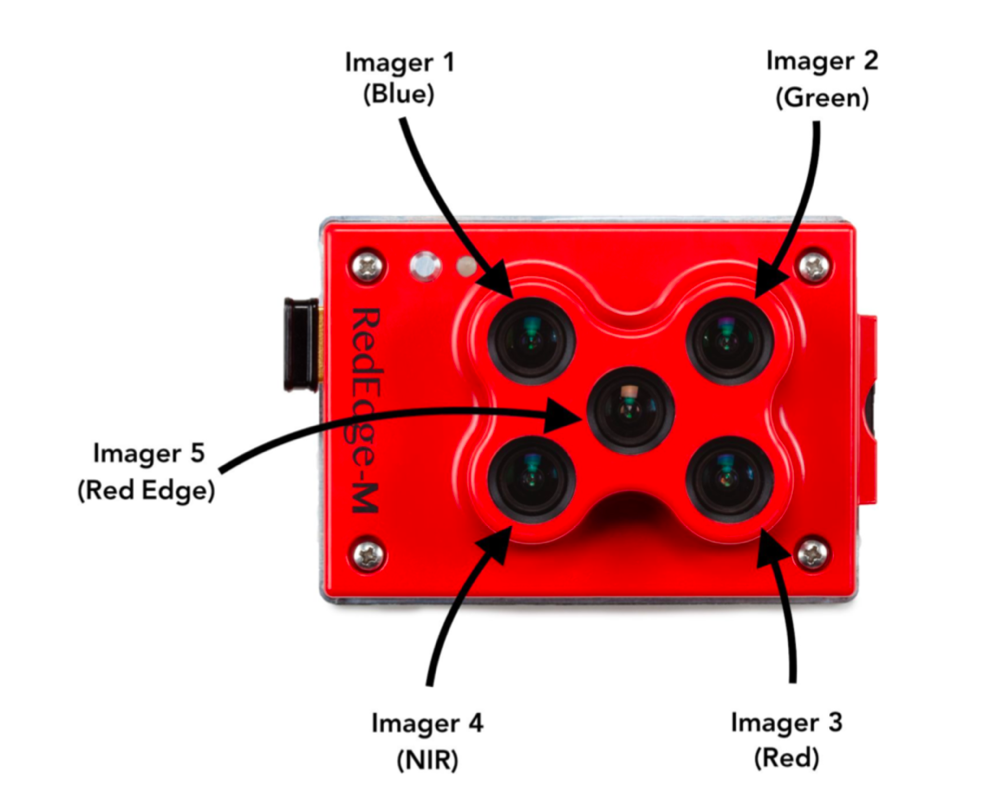
\includegraphics[width=8 cm]{micasense.png}
	
\end{figure}

\begin{figure}[H]
	\centering
	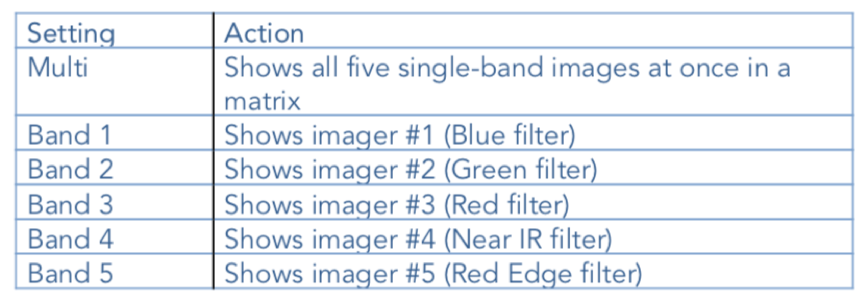
\includegraphics[width=8 cm]{micasense1.png}
	
\end{figure}

The RedEdge-M camera stores files in a folder structure and within each, a subfolder with the images themselves is created. If more than 200 images are stored, a second image folder is created ($'000'$ and $'001'$ for instance). 
Two log files are also created for each camera power cycle. Within each subfolder a group of 5 files is created for each image capture (.tif)
The .tif files are 12-bit resolution stored in either 12-bit DNG RAW format or 16-bit .tif RAW format depending on the setting. The resolution is 1280x960 pixels and the metadata tags are embedded for each file in standard EXIF format.

\begin{figure}[H]
	\centering
	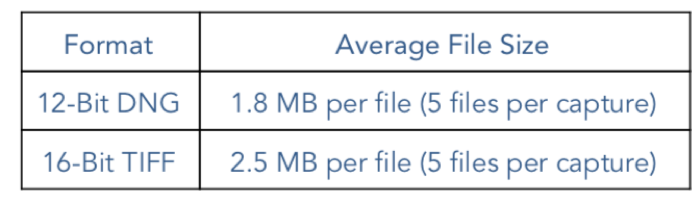
\includegraphics[width=8 cm]{micasense2.png}
	
\end{figure}

\section*{First Step: Image Alignment}
In a typical image alignment problem we have two images of a scene, related by a motion model. Different image alignment algorithms aim to estimate the parameters of these motion models using different tricks and assumptions.
The OpenCV constants that represent these models have a prefix $MOTION$.
An Affine transform is stored in a 2 x 3 sized matrix. Translation and Euclidean transforms are special cases of the Affine transform. In Translation, the rotation, scale and shear parameters are zero, while in a Euclidean transform the scale and shear parameters are zero. So Translation and Euclidean transforms are also stored in a 2 x 3 matrix. Once this matrix is estimated, the images can be brought into alignment using the function warpAffine.
Homography, on the other hand, is stored in a 3 x 3 matrix. Once the Homography is estimated, the images can be brought into alignment using warpPerspective.
A new measure of similarity is proposed, called Enhanced Correlation Coefficient (ECC) for estimating the parameters of the motion model. The advantage is that unlike the traditional similarity measure of difference in pixel intensities, ECC is invariant to photometric distortions in contrast and brightness.
In OpenCV the motion model for ECC image alignment is estimated using the function $findTransformECC$.
Here are the steps for using this function:
\begin{enumerate}
\item Read the images
\item Convert them to grayscale
\item Pick a motion model you want to estimate
\item Allocate space ($warp\_matrix$) to store the motion model
\item Define a termination criteria that tells the algorithm when to stop
\item Estimate the $warp\_matrix$ using $findTransformECC$
\item Apply the $warp\_matrix$ to one of the images to align it with the other image
\end{enumerate}

\section*{Second Step: NDVI}
The NDVI is a dimensionless index that describes the difference between visible and near-infrared reflectance of vegetation cover and can be used to estimate the density of green on an area of land.
The NDVI is calculated from reflectance measurements in the red and near infrared (NIR) portion of the spectrum:
\begin{equation}
NDVI = \dfrac{R_{NIR} - R_{RED}}{R_{NIR} + R_{RED}}
\end{equation}
where $R_{NIR}$ is the reflectance of NIR radiation and $R_{RED}$ is the reflectance of visible red radiation.
This index defines values from $-1.0$ to $1.0$ basically representing greens where negative values are mainly formed from clouds, water and snow, and values close to zero are primarily formed from rocks and bare soil. Very small values ($0.1$ or less) of the NDVI function correspond to empty areas of rocks, sand or snow. Moderate values (from $0.2$ to $0.3$) represent shrubs and meadows, while large values (from $0.6$ to $0.8$) indicate temperate and tropical forests. 
Put simply, NDVI is a measure of the state of plant health based on how the plant reflects light at certain frequencies (some waves are absorbed and others are reflected).

\section*{Third Step: K-means Clustering}
Clustering is one of the most common exploratory data analysis technique used to get an intuition about the structure of the data. It has the task of identifying subgroups in the data such that data points in the same subgroup (cluster) are very similar, while data points in different clusters are very different.
The algorithm we are going to use is the K-means which tries to partition the dataset into $K$ predefined distinct non-overlapping subgroups where each data point belongs to only one group.
Here are the steps for using this algorithm:
\begin{enumerate}
\item Clusters the data into $K$ groups where $K$  is predefined
\item Select $K$ points at random as cluster centers
\item Assign objects to their closest cluster center according to the Euclidean distance function
\item Calculate the centroid or mean of all objects in each cluster
\item Repeat steps 2, 3 and 4 until the same points are assigned to each cluster in consecutive rounds
\end{enumerate}
\newpage
\section*{Images of the results}
\begin{figure}[H]
	\centering
	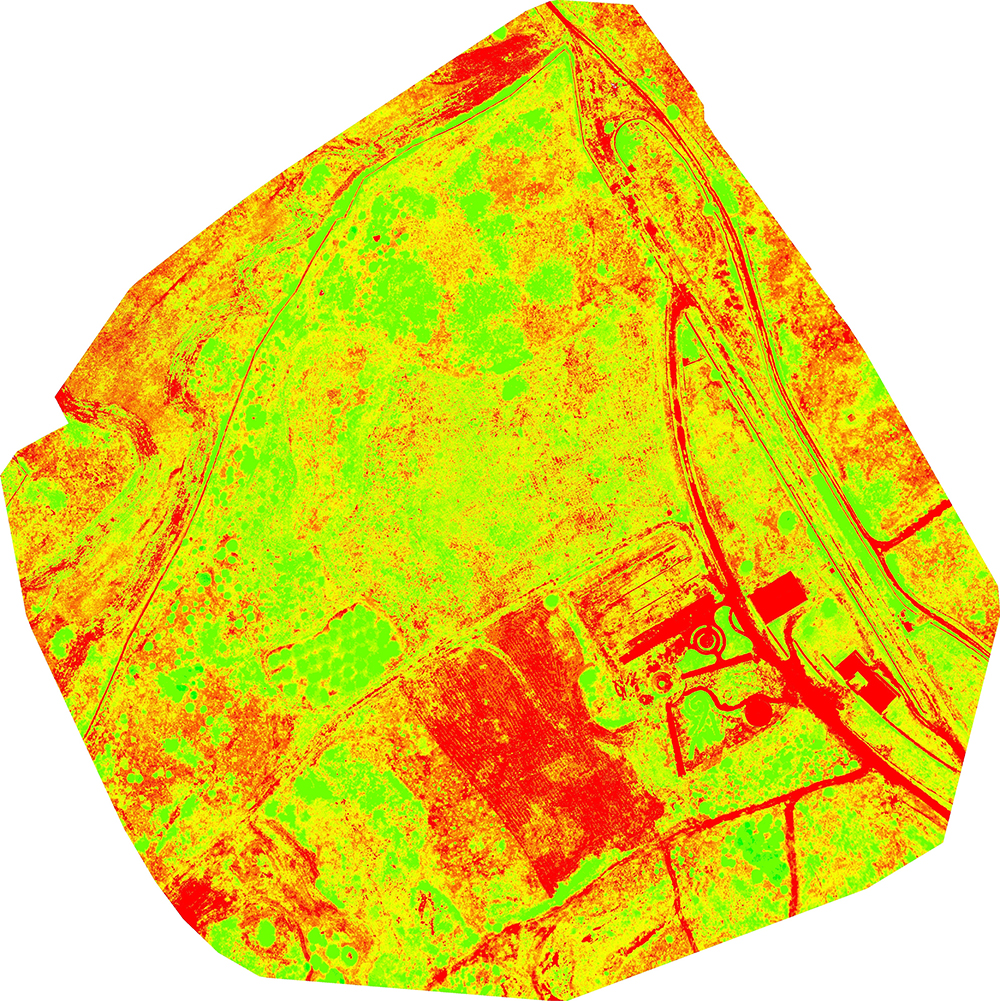
\includegraphics[width=8 cm]{ortobotanicondvi.jpg}
	\caption{NDVI botanical garden University of Salento}
\end{figure}

\begin{figure}[H]
	\centering
	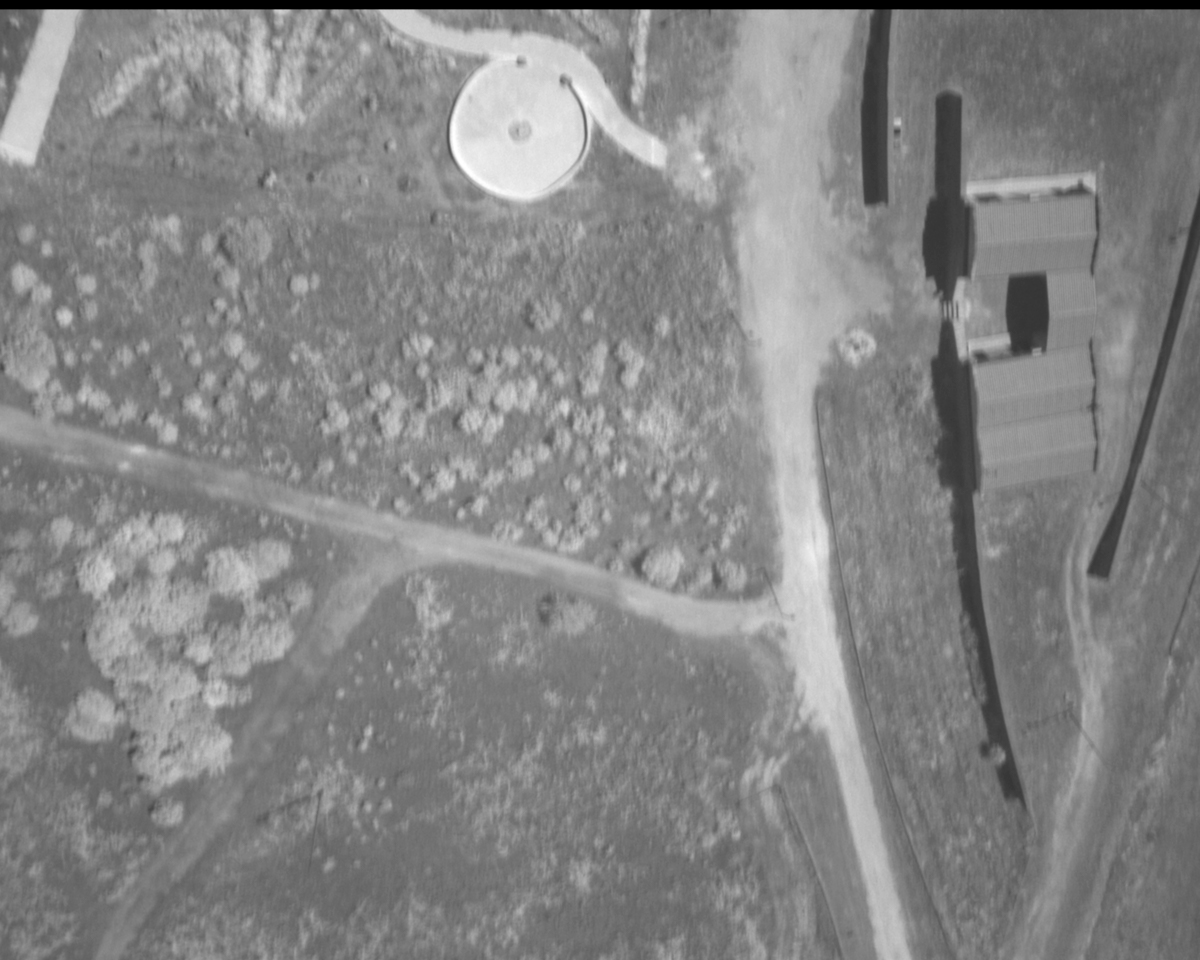
\includegraphics[width=9 cm]{niraligned.jpg}
	\caption{Aligned NIR image}
\end{figure}

\begin{figure}[H]
	\centering
	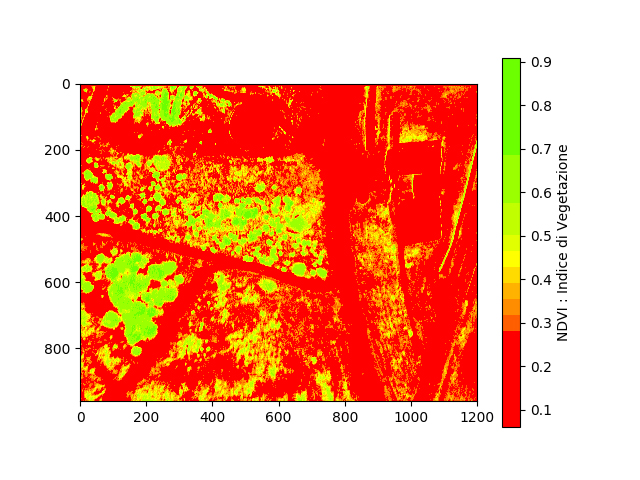
\includegraphics[width=12 cm]{NDVI.jpg}
	\caption{NDVI}
\end{figure}

\begin{figure}[H]
	\centering
	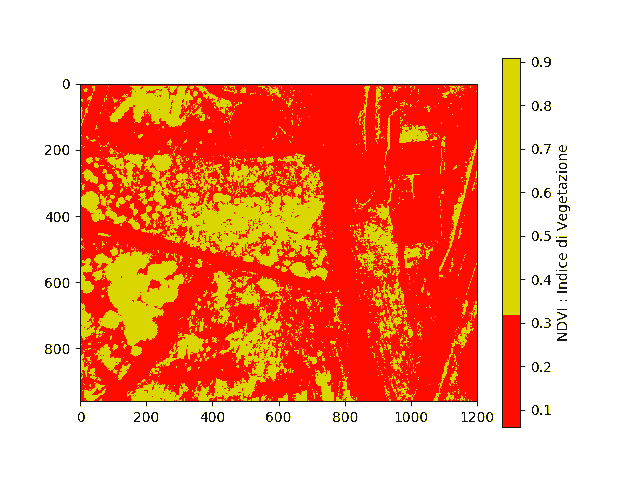
\includegraphics[width=12 cm]{clusteringNDVI.jpg}
	\caption{Clustering NDVI with $K=4$}
\end{figure}

\end{document}
